\section{Design of the System}
\label{sec:SystemDesign}


%later convert this pdf
\begin{figure}[t]
\centering
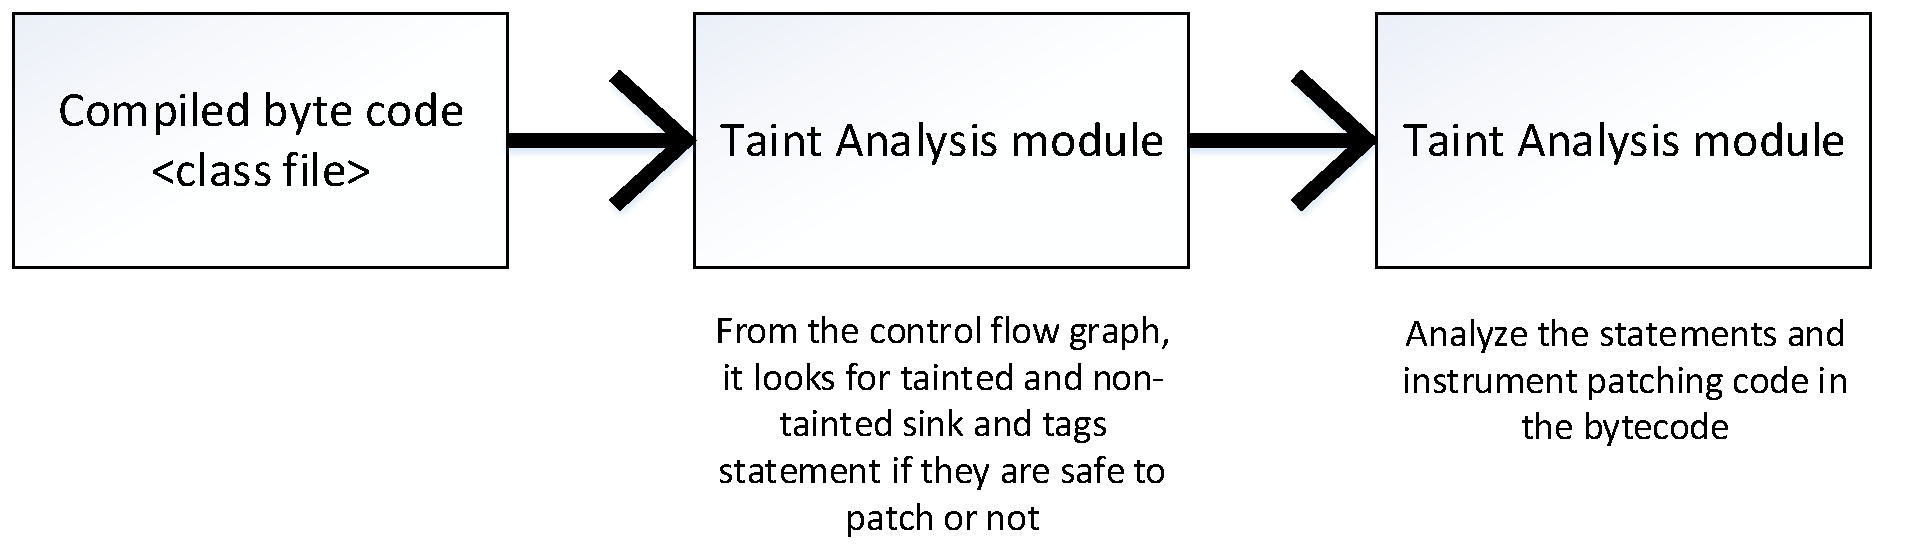
\includegraphics[width=3.2in]{images/OverallDesign.png}
\caption{Overall Design}
\label{fig:overallDesign}
\end{figure}


% \begin{figure}[!htb]
% \centering
% 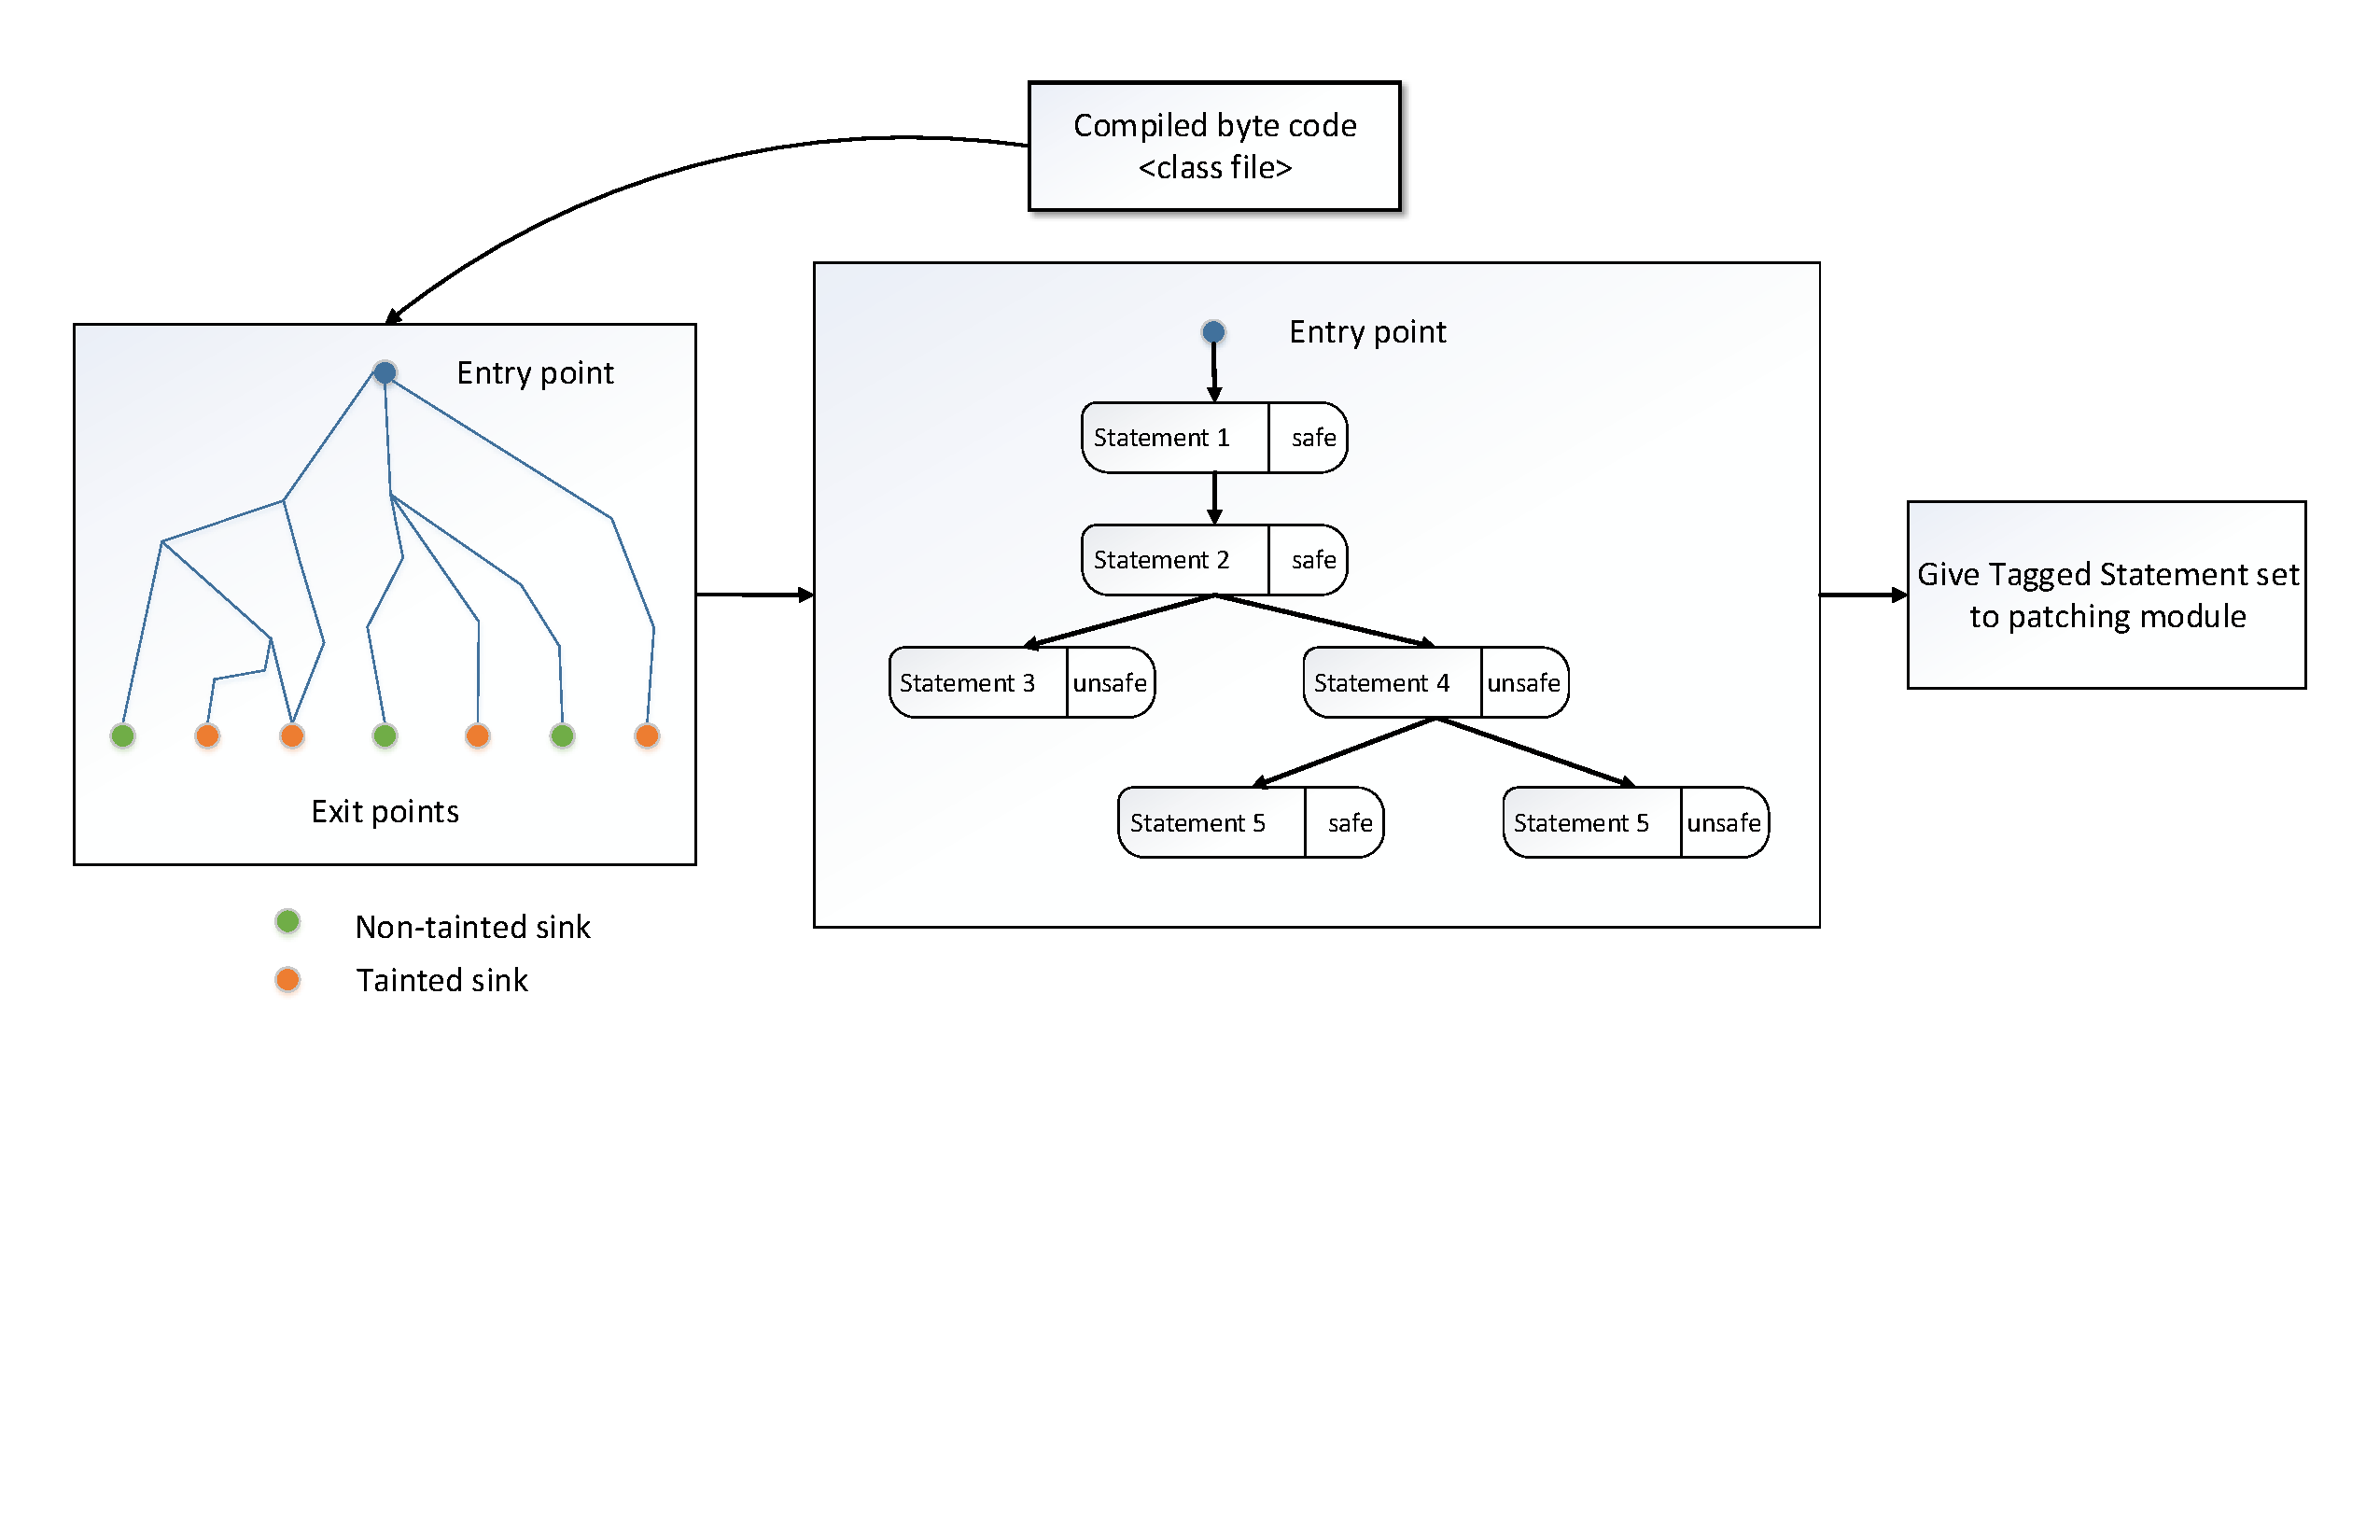
\includegraphics[width=3.5in]{images/TaintModule.pdf}
% \caption{Overall Design}
% \label{fig:TaintModule}
% \end{figure}
% 
% \begin{figure*
%   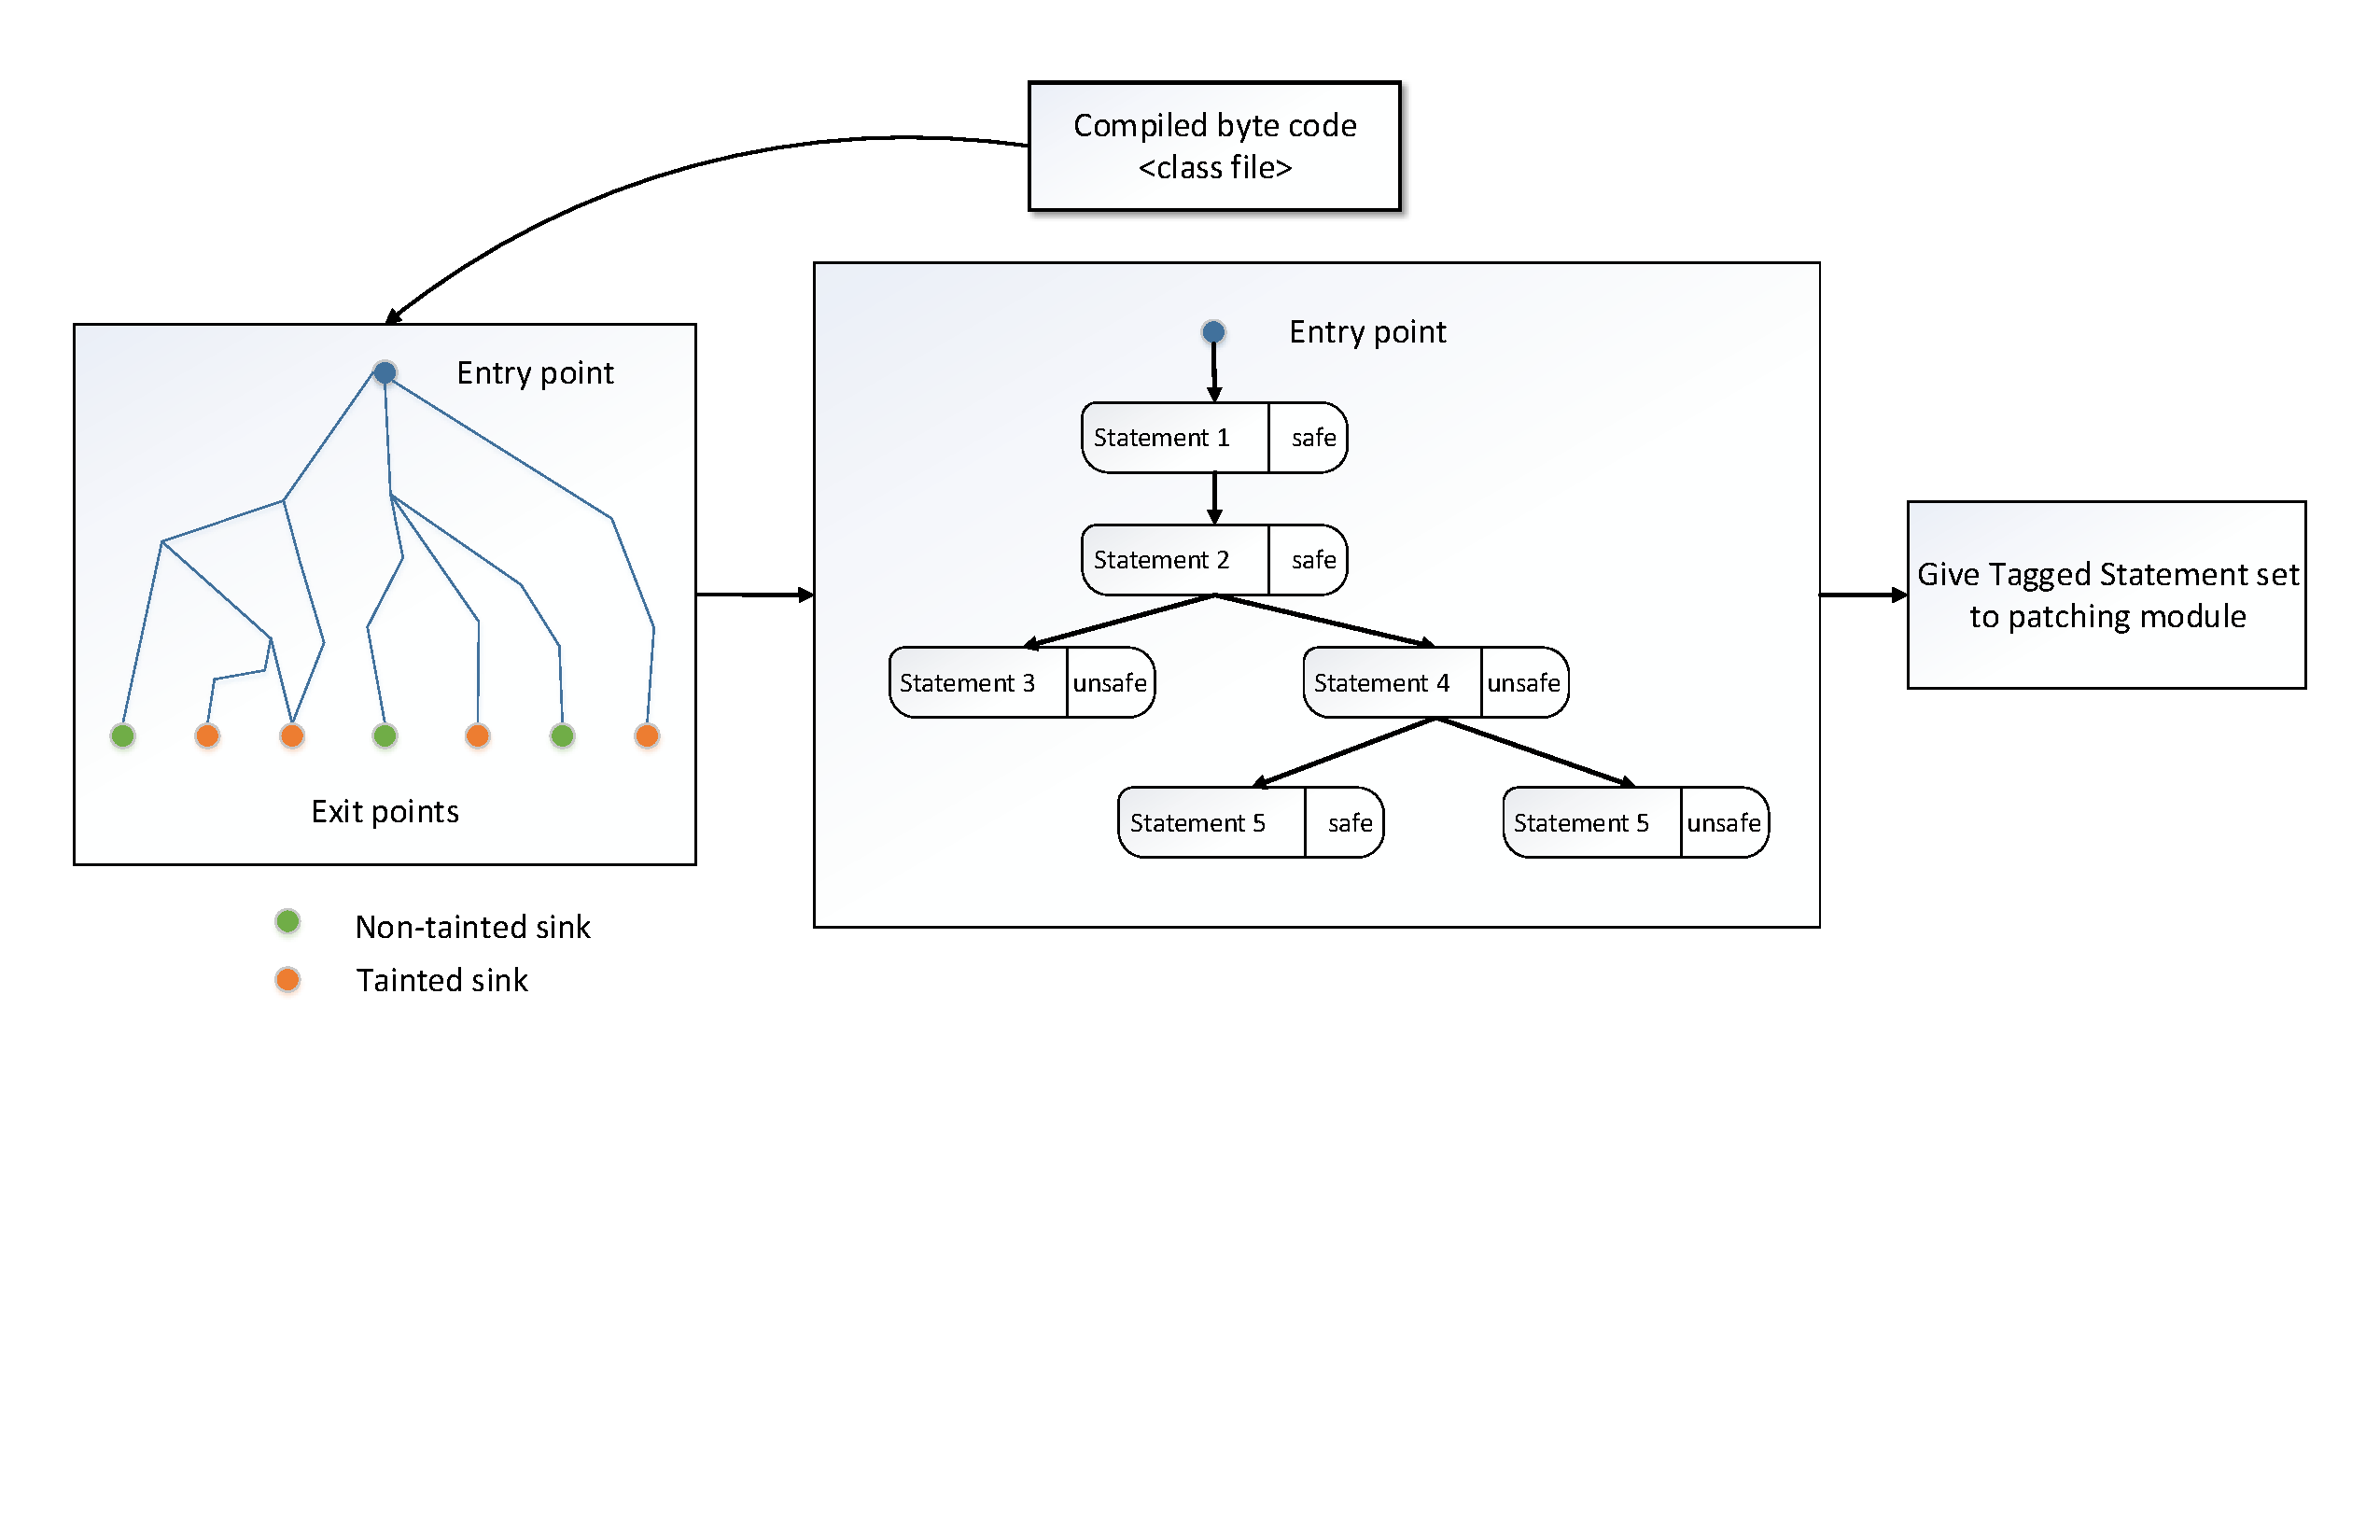
\includegraphics[width=\textwidth,height=5cm]{images/TaintModule.pdf}
%   \caption{Design of the Taint Module}
% \end{figure*}

%later covert this to pdf
\begin{figure*}[t]
\centering
  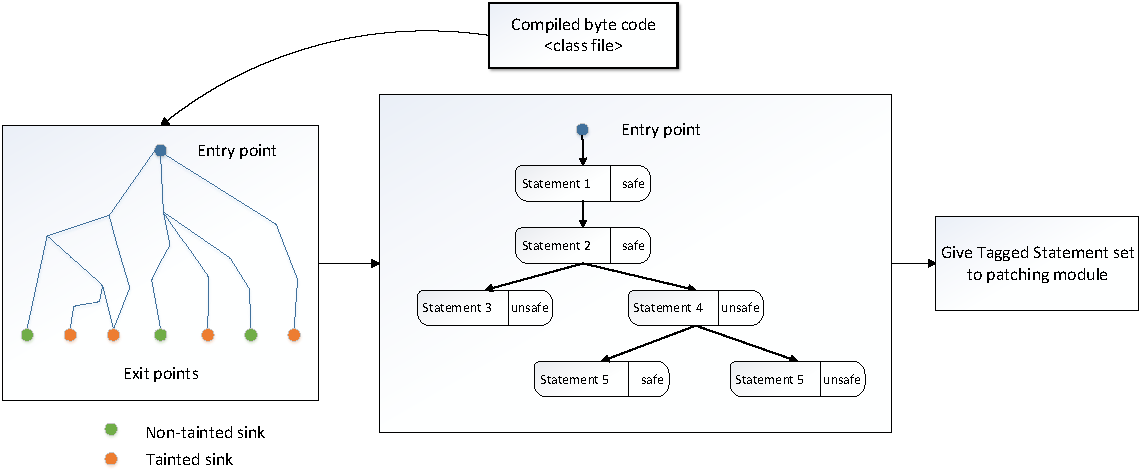
\includegraphics[width= 7.0in]{images/TaintModule.png}
  \caption{Design of the Taint Module}
  \label{fig:TaintModule}
\end{figure*}


The overall design of the repairing framework is illustrated in
Figure~\ref{fig:overallDesign}. The framework consists of two basic modules.


\subsection{Taint analysis Module}
\label{subsec:TaintModule}

The main purpose of the taint analysis module is to classify which of the
statements are safe to patch or not. Based on the analysis result in this
module, the tagged statement will be passed to the repairing module.


We have specify the list of source, sink and derivation methods in a
configuration file before the analysis. The source methods includes methods
which
take input from user from console or web application forms like text box. The
sink methods are sensitive data storage which are unsafe to manipulate such as
database, console print or methods to send a text file to printer etc. The
overview of the taint analysis module is illustrated in the
Figure~\ref{fig:TaintModule}.  The input for the module is the compiled byte
code intended to be repaired. Here we have generated a control flow graph (CFG)
from the class file to get all the possible program paths. Here a point to be
noted that any modification along the path going to the tainted sink is unsafe
to patch.


\subsubsection{Tainting Rules}
\label{subsubsec:TaintingRule}
\textcolor{red}{\textbf{Needs Revision}}\newline

\begin{table}[t]
\centering
\small
\begin{tabular}{l|l}
\multicolumn{1}{c|}{\textbf{\java\ Class}} & \multicolumn{1}{c}{\textbf{Source
Method}}\\
% \scalebox{0.86}
% {
\hline
\code{java.io.InputStream} & \code{read()}\\
\code{java.io.BufferedReader} & \code{readLine()}\\
\code{java.net.URL} & \code{openConnection()}\\
\code{org.apache.http.HttpResponse} & \code{getEntity()}\\
\code{org.apache.http.util.EntityUtils} & \code{toString()}\\
\code{org.apache.http.util.EntityUtils} & \code{toByteArray()}\\
\code{org.apache.http.util.EntityUtils} & \code{getContentCharSet()}\\
\code{javax.servlet.http.HttpServletRequest} & \code{getParameter()}\\
\code{javax.servlet.ServletRequest} & \code{getParameter()}\\
\code{java.Util.Scanner} & \code{next()}\\
\end{tabular}
\caption{Common \java\ library taint source functions}
\label{tab:TaintSources}
% }
\end{table}



\begin{table}[t]
\centering
\small
\begin{tabular}{l|l}
\multicolumn{1}{c|}{\textbf{\java\ Class}} & \multicolumn{1}{c}{\textbf{Sink
Method}}\\
% \scalebox{0.86}
% {
\hline
\code{java.io.PrintStream} & \code{printf()}\\
\code{java.io.OutputStream} & \code{write()}\\
\code{java.io.FileOutputStream} & \code{write()}\\
\code{java.io.Writer} & \code{write()}\\
\code{java.net.Socket} & \code{connect()}\\
%org.apache.http.impl.client.DefaultHttpClient & execute\\ \hline
\end{tabular}
% }
\caption{Common \java\ library taint sink functions}
\label{tab:TaintSinks}
\end{table}


We have used extended InFlow framework for the taint analysis module. The steps
are

\begin{mylist}
  \item We defined list of source and sink taint methods listed in
  Table~\ref{tab:TaintSources} and \ref{tab:TaintSinks}. We are only tainting
  the variables which are coming from the listed taint source methods.
  
  \item We have also listed all taint propagation methods. The assignment ($=$)
  is the basic taint propagator. But there are other methods like \code{append}
  in \code{java.lang.StringBuffer} and \code{java.lang.StringBuilder} which are
  taint propagator.

  \item All the variable which are referred to tainted variables/ objects or
  output of taint propagator over tainted variable/objects are also considered
  as tainted.

  \item For all the program patch we see if such tainted variables are reaching
  the tainted sink or not. If they are reaching to some tainted sink then all
  the statements along that particular program path to which the tainted
  variables are assigned are marked as unsafe otherwise safe.
\end{mylist}


\subsection{Repairing Module}
\label{subsec:RepairingModule}

%later covert this to pdf
\begin{figure}[t]
\centering
  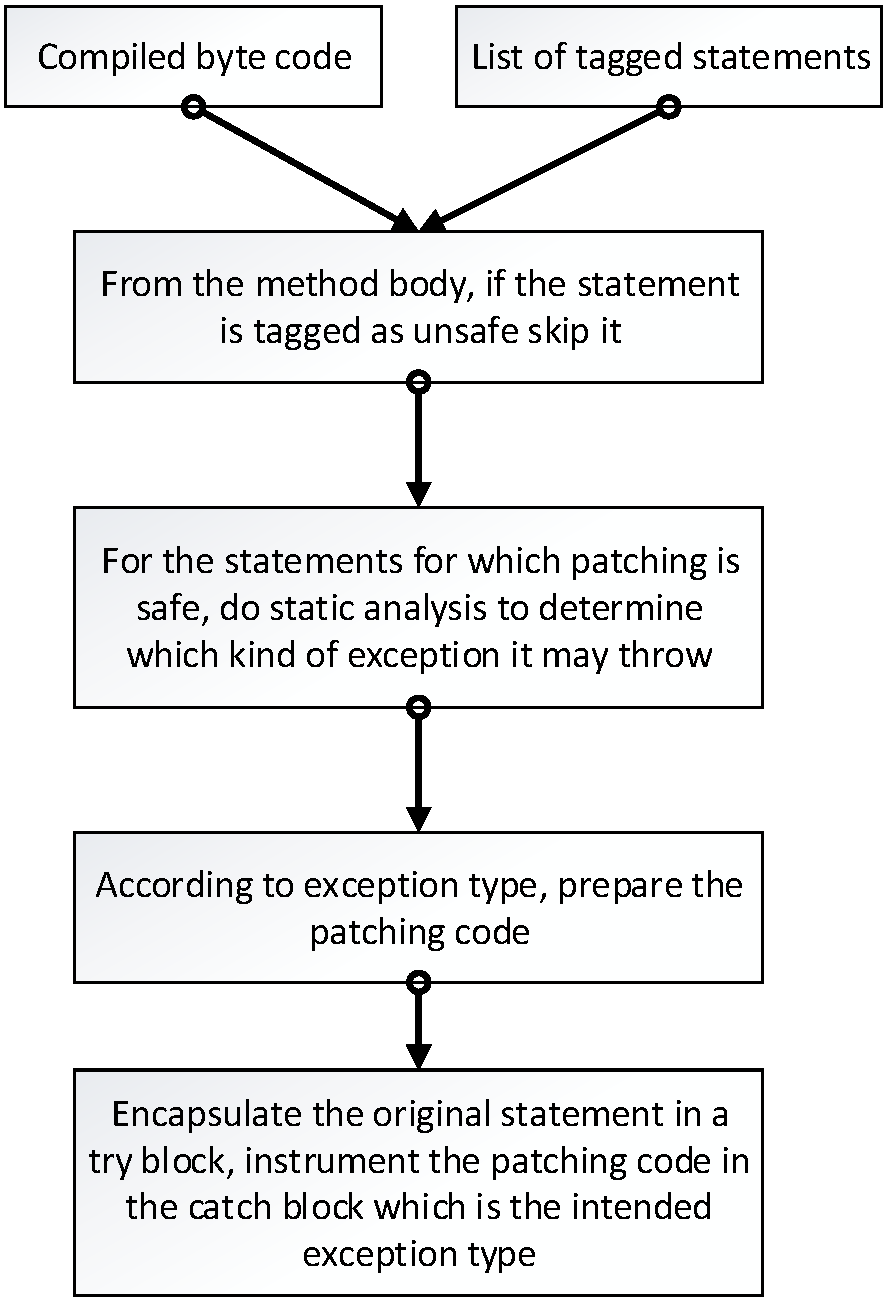
\includegraphics[scale= .5]{images/PatchModule.png}
  \caption{Design of the Patching Module}
  \label{fig:PatchModule}
\end{figure}

The repairing module is consisted of three phases. All these three phases
requires three sequential passes over the input bytecodes to produce the final
patched result.


\subsubsection{Method Shilding}
\label{MethodShilding}


When we are shielding a method, we also looked to the calling context of that
particular method. The method can be called from a path which leads to some
tainted sink and it can also be called from such path which does not contain
any taint sink. In such cases, we have taken special care about the callee. The
path to the tainted sink should not call a patched method as it can influence
data which are leaving the system. So, we also maintained two different version
of
the method and instrument the calling site so that appropriate method is called.

\lstset{language=java, caption = Same method calling in different scenario,
label=callingContext}
\begin{figure}[t]
\begin{lstlisting}[countblanklines=false]
int bar(int a, int b) {
    return a/b;
}
void foo() {
    int a = 10, b = 0, c = 15;
    int out = bar(a, b);
    TaintSink(out);
    int out1 = bar(c, b);
    NonTaintSink(out1);
}
\end{lstlisting}
\end{figure}

\lstset{language=java, caption = Method name modification for different calling
context, label=callingContextPatch}
\begin{figure}[t]
\begin{lstlisting}[countblanklines=false]
int bar(int a, int b) {
    return a/b;
}
int bar_untainted_fa844d57(int a, int b) {
    int out;
    try {
	out = a/b;
    } catch(ArithmeticException ex) {
	b = 1;
	out = a/b;
    }
    return out;
}
void foo() {
    int a = 10, b = 0, c = 15;

    // no modification in the call where the result can go to a tainted sink
    // method
    int out = bar(a, b);
    TaintSink(out);

    // Modify the method call to the shielded method as the result is not going
    // to any tainted sink method
    int out1 = bar_untainted_fa844d57(c, b);
    NonTaintSink(out1);
}
\end{lstlisting}
\end{figure}

In the Listing~\ref{callingContext} and \ref{callingContextPatch} we have
defined an example code snippet of the original code and the patched code where
we have renamed the method \emph{bar} to \emph{bar\_untainted\_fa844d57}
before instrumenting any patching code in it. The variable \emph{out} goes to a
tainted sink while \emph{out1} does not. So the we have done modification in the
line where \emph{out1} is defined. As \emph{out} is going to a tainted sink
method, we did not do any modification to it.



% \begin{enumerate}
%   \item \textbf{Taint analysis module :}
%   \item \textbf{Repairing Module : }
% \end{enumerate}
